\section{CCVPN Design}\label{metho}

Traditional Virtual Private Networks (VPNs) extend private networks across the Internet. They enable users to send and receive data across shared or public networks as if their computing devices were directly connected to the same private network~\cite{khanvilkar2004virtual}. The goal of CCVPN it to provide its users with the same functionality within the CCN Internet architecture. Therefore, the users can benefit from the features and security of a private network, even though the are not physically under the same private network.

In CCVPN, there are four main entities involved in the virtual private communication: \textit{Consumer}, \textit{Producer}, \textit{Consumer Side Gateway} ($G_c$), and \textit{Producer Side Gateway} ($G_p$). As in usual CCNs, the \textit{Consumer} is the network node that issues an interest for a given content (e.g., file, web page, video) that it wishes to retrieve. The Producer is the network node which originally created such content. $G_c$ and $G_p$ are the edge gateways responsible for ensuring the private communication among distinct domains. As we discuss later on, $G_c$ and $G_p$ can actually be implemented as a single network device, but we firstly present them as separate entities for the purpose of clarity.

\begin{figure*}[!ht]
\centering
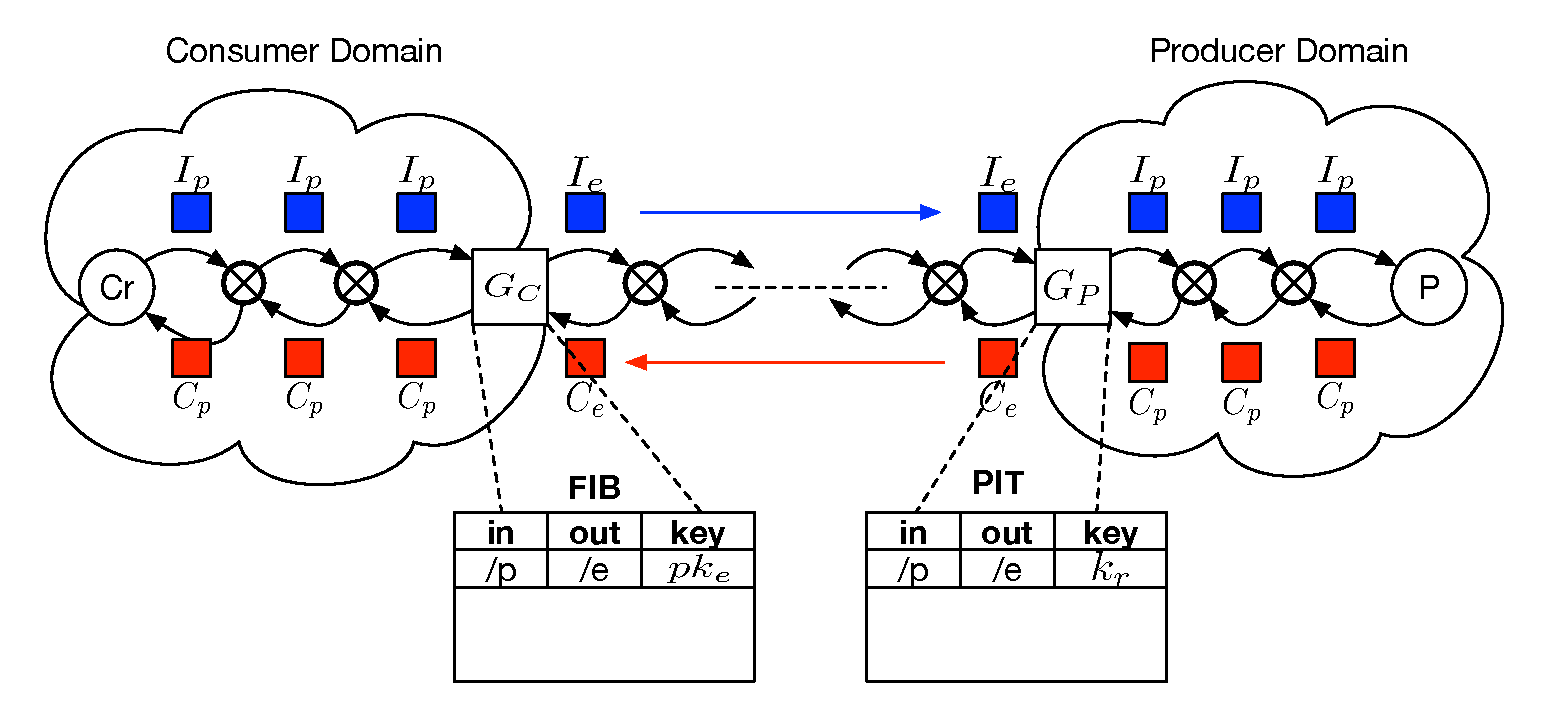
\includegraphics[width=1.9\columnwidth]{images/architecture.pdf}
\caption{CCVPN connectivity architecture}
\label{fig:ccvpn}
\end{figure*}

As depicted in Fig.~\ref{fig:ccvpn}, the devices inside the \textit{Consumer} domain form a physically interconnected private network. Conversely, the devices in the \textit{Producer} domain also form a private network. Therefore, the goal is to create an overlay virtual network that unifies the \textit{Consumer} and the \textit{Producer} domains in way such that the original interests and contents are only visible to the devices inside these two domains. In other words, the interest $I_e$ and the content $C_e$, that are forwarded outside these domains, should give no information about the original interest $I_p$ and the actual content $C_p$.

In order to achieve such anonymous communication, $G_c$ is introduced in the \textit{Consumer} domain to encapsulate outgoing interests. Conversely, the $G_p$ is responsible for decapsulating the incoming encapsulated interests and forwarding them in their original form. When the content is forwarded back in response to the interest, $G_p$ encrypts the content before sending it outside the \textit{Producer} domain. Finally, $G_c$ decrypts the received content to its original form and forwards it back towards the \textit{Consumer}. Through the rest of this section we provide a detailed description on how such actions are implemented.

Upon the arrival of a new interest $I_p$, $G_c$ checks its Forwarding Information Base (FIB) to check if the interest prefix is in the list of prefixes for VPN communication. We assume that the FIB must be pre-configured with the list of prefixes which will trigger the VPN communication. Associated with such prefixes are $G_p$'s name and public key ($pk_e$). Therefore, if the prefix of $I_p$ is in the VPN prefixes list, $G_P$ runs Algorithm~\ref{alg:interestEncap} to generate a new interest $I_e$ which encapsulates the original interest $I_p$. Firstly, Algorithm~\ref{alg:interestEncap} generates a random symmetric key ($k_r$) which will be used later on to perform the \textit{Content} Encryption/Decryption. Next, it retrieves $G_p$'s name and public key from the FIB. It uses the public key to encrypt the symmetric key $k_r$ and the original interest $I_p$. Then it creates the new interest $I_e$ with $G_p$'s name as the interest name and the generated ciphertext as payload. Since $I_e$ has  the $G_p$'s name it will be routed towards $G_p$ and since the payload is singed with $G_p$'s public key, only $G_p$ can retrieve the original interest $I_p$ and the symmetric key $k_r$.

\begin{algorithm}[]\label{alg:interestEncap}
\SetKwInOut{Input}{input}
\SetKwInOut{Output}{output}
\Input{Original interest $I_p$;}
\Output{Encapsulated interest $I_e$;}
%$Ip_{name}$ = getName($I_p$)\\
%storeToPIT($Ip_{name}$)\\
$k_r$ = symmKeyGen();\\
$Gp_{name}$ = retrieveNameFromFIB($I_p$)\\
$pk_e$ = retrievePKFromFIB($I_p$)\\
$payload$ = $Enc_{pk_e}(I_p||k_r)$\\
$I_e$ = createNewInterest($Gp_{name}$, $payload$)\\
storeToPIT($I_e$,$k_r$)\\
\Return $I_e$;\\
\caption{Interest encapsulation (runs on $G_c$)}
\end{algorithm}

After the message is routed towards $G_p$, $G_p$ verifies if the incoming interest name prefix matches its own name and, if it does, $G_p$ runs Algorithm~\ref{alg:interestDecap}, using its own secret key ($sk_e$) to decrypt $I_e$'s payload, which results in the original interest $I_p$ and the symmetric key $k_r$. $G_p$ then stores $I_e$'s name and the symmetric key $k_r$ in its own PIT, within the entry for the pending interest $I_p$, and forwards $I_p$. $I_e$'s name and $k_r$ are stored so that they can be used later on to generate the encrypted content $C_e$.

\begin{algorithm}[]\label{alg:interestDecap}
\SetKwInOut{Input}{input}
\SetKwInOut{Output}{output}
\Input{ Encapsulated interest $I_e$;}
\Input{ Private key $sk_e$;}
\Output{Original interest $I_p$;}
$Ie_{name}$ = getName($I_e$)\\
$cipherText$ = getPayload($I_e$)\\
$I_p||k_r$ = $Dec_{sk_e}(cipherText)$\\
storeToPIT($I_p$,$k_r$,$Ie_{name}$)\\
\Return $I_p$;\\
\caption{Interest decapsulation (runs on $G_p$)}
\end{algorithm}

The original interest $I_p$ is forwarded inside the \textit{Producer} domain until it reaches the \textit{Producer}. The \textit{Producer} responds with the content $C_p$ which is forwarded back to $G_p$.
Upon receiving $C_p$, $G_p$ fetches for $C_p$'s name (which is equal to $I_p$'s name) on its PIT, retrieving $k_r$ and $Ie$'s name. Then it uses $k_r$ to encrypt-then-MAC the real content response $C_p$ and creates $C_e$ which must have the same name as $I_e$ and the encryption of $C_p$ as payload (Algorithm~\ref{alg:contentEnc}). Since only $G_c$ and $G_p$ share the symmetric key $k_r$, only $G_c$ will be able to decrypt $C_e$'s payload into $C_p$. Therefore nobody from outside the VPN is able to access the content nor the Producer's identity.

\begin{algorithm}[]\label{alg:contentEnc}
\SetKwInOut{Input}{input}
\SetKwInOut{Output}{output}
\Input{Original content $C_p$;}
\Output{Encrypted content $C_e$;}
$name$ = getName($C_p$)\\
$k_r$ = retrieveKeyFromPIT($name$)\\
$Ie_{name}$ = retrieveNameFromPIT($name$)\\
$payload$ = EncryptThenMAC($k_r$,$C_p$)\\
$C_e$ = createNewContent($Ie_{name}$,$payload$)\\
\Return $C_e$;\\
\caption{Content encryption  (runs on $G_p$)}
\end{algorithm}

Since $C_e$ and $I_e$ have the same name, $C_e$ will be forwarded all the way back to $G_c$. When $G_c$  receives $C_e$ $G_c$ will execute Algorithm~\ref{alg:contentDec}. It will match $C_e$'s name to the pending interest $I_e$ in its PIT, retrieving $k_r$. $k_r$ can then be used to verify the integrity of the received content and to decrypt it into the actual content $C_p$. After that, $C_p$ can be forwarded back to the \textit{Consumer}. If the MAC verification fails, it means that $C_e$ has been forged and $G_c$ ignores it.

\begin{algorithm}[]\label{alg:contentDec}
\SetKwInOut{Input}{input}
\SetKwInOut{Output}{output}
\Input{Encrypted content $C_e$;}
\Output{Original content $C_p$;}
$Ce_{name}$ = getName($C_e$)\\
$k_r$ = retrieveKeyFromPIT($Ce_{name}$)\\
$cipherText$ = getPayload($C_e$)\\
$C_p$ = Dec($k_r$,$cipherText$)\\
\eIf{$C_p$ == $\perp$}
    {
    \tcc{MAC verification failed}
    \Return ;\\
    }
    {\Return $C_p$;\\}
\caption{Content decryption (runs on $G_c$)}
\end{algorithm}

For clarity, we have defined a \textit{Consumer} and a \textit{Producer} domain. However, in reality, a single gateway can implement the functions of both $G_c$ and $G_p$. Therefore, consumers and producers can exist in both the domains and interests for contents can be issued from both sides. Also, it is worth to mention that, within the created CCVPNs, content caching would work just as it works in regular CCNs,  i.e., routers would be able to cache contents and respond to interests that were previously requested, enabling better resource usage and lower communication delays. Finally, we emphasize that $G_c$ encapsulation and decryption functions can also run inside the Consumer host. Conversely, $G_p$ can be implemented within the \textit{Producer} host. This enables its usage for one-to-one communication that would be completely anonymous to any  other entity in the network.
